% =====================================================================
% COMP4620/8620 - Advanced Topics in AI: Intelligent Robotics
% Semester 2 2026 - Assignment 2 report template
% Compile: pdflatex a2_report.tex (run twice for references)
% Submit the PDF together with a .zip/.7z/.tar.gz of code + test cases.
% =====================================================================
\documentclass[11pt,a4paper]{article}

\usepackage[margin=2.2cm]{geometry}
\usepackage{amsmath,amssymb,amsthm}
\usepackage{graphicx}
\usepackage{booktabs}
\usepackage{multirow}
\usepackage{xcolor}
\usepackage{enumitem}
\usepackage{hyperref}
\usepackage[ruled,vlined,linesnumbered]{algorithm2e}
\usepackage{listings}
\usepackage{float}
\usepackage{subcaption}

\hypersetup{colorlinks=true, linkcolor=blue!50!black, urlcolor=blue!50!black, citecolor=blue!50!black}
\lstset{basicstyle=\ttfamily\small, breaklines=true, frame=single, columns=fullflexible}

% Placeholder marker - search for \todo and remove before submitting
\newcommand{\todo}[1]{\textcolor{red}{\textbf{[TODO: #1]}}}
\newcommand{\R}{\mathbb{R}}
\newcommand{\E}{\mathbb{E}}

\title{COMP4620/8620 Advanced Topics in AI: Intelligent Robotics\\
       Assignment 2 Report}
\author{Hadis Amin - u8050066}
\date{}

\begin{document}
\maketitle


% =====================================================================
\section*{Part A}
% =====================================================================

% ---------------------------------------------------------------------
\subsection*{A1. State abstraction of the 1-D grid MDP}

No. Abstracting the state into $L$ and $R$ does not turn this into an MDP. An MDP assumes the agent knows exactly which state it is in. Here the true state is still uncertain: we only believe the agent is somewhere on the left side or the right side, not exactly where. The agent therefore still needs a belief, a probability distribution over the possible states, so the problem remains a POMDP.

% ---------------------------------------------------------------------
\subsection*{A2. $\alpha$-vector policy representation}

Let $b = (p, 1-p)$ where $p = b(s_1)\in[0,1]$. Then
$\alpha\cdot b = \alpha(s_1)\,p + \alpha(s_2)\,(1-p)$.

\begin{table}[H]
\centering
\begin{tabular}{lcc}
\toprule
$\alpha$ & vector & $V_\alpha(p) = \alpha\cdot b$ \\
\midrule
$\alpha_1$ & $[10,-5]$  & $15p - 5$ \\
$\alpha_2$ & $[-5,10]$  & $-15p + 10$ \\
$\alpha_3$ & $[4,4]$    & $4$ \\
$\alpha_4$ & $[1,2]$    & $-p + 2$ \\
$\alpha_5$ & $[5.5,1]$  & $4.5p + 1$ \\
\bottomrule
\end{tabular}
\caption{Value of each $\alpha$-vector as a function of $p=b(s_1)$.}
\end{table}

\paragraph{(a) Belief intervals where each $\alpha$-vector is maximal.}
Figure~\ref{fig:alpha-vectors} plots the five lines over $p\in[0,1]$. The shaded upper surface is made of three segments: $\alpha_2$ on the left, $\alpha_3$ in the middle and $\alpha_1$ on the right. The breakpoints (marked in the figure) are the intersections
$\alpha_2 = \alpha_3 \Rightarrow -15p + 10 = 4 \Rightarrow p = 0.4$ and
$\alpha_3 = \alpha_1 \Rightarrow 15p - 5 = 4 \Rightarrow p = 0.6$.
The figure also shows that $\alpha_4$ and $\alpha_5$ lie strictly below the surface everywhere: $\alpha_4$ never exceeds $2 < 4$, and $\alpha_5$ is below $\alpha_3$ on $[0, 2/3)$ and below $\alpha_1$ for $p > 4/7$, so neither is ever maximal. The resulting intervals are summarised in Table~\ref{tab:alpha-intervals}.
\begin{table}[H]
\centering
\begin{tabular}{lc}
\toprule
$\alpha$ & Interval of $p=b(s_1)$ where maximal \\
\midrule
$\alpha_1$ & $[0.6,\, 1]$ \\
$\alpha_2$ & $[0,\, 0.4]$ \\
$\alpha_3$ & $[0.4,\, 0.6]$ \\
$\alpha_4$ & never \\
$\alpha_5$ & never \\
\bottomrule
\end{tabular}
\caption{Belief intervals where each $\alpha$-vector is maximal (read off Figure~\ref{fig:alpha-vectors}).}
\label{tab:alpha-intervals}
\end{table}
\begin{figure}[H]\centering
  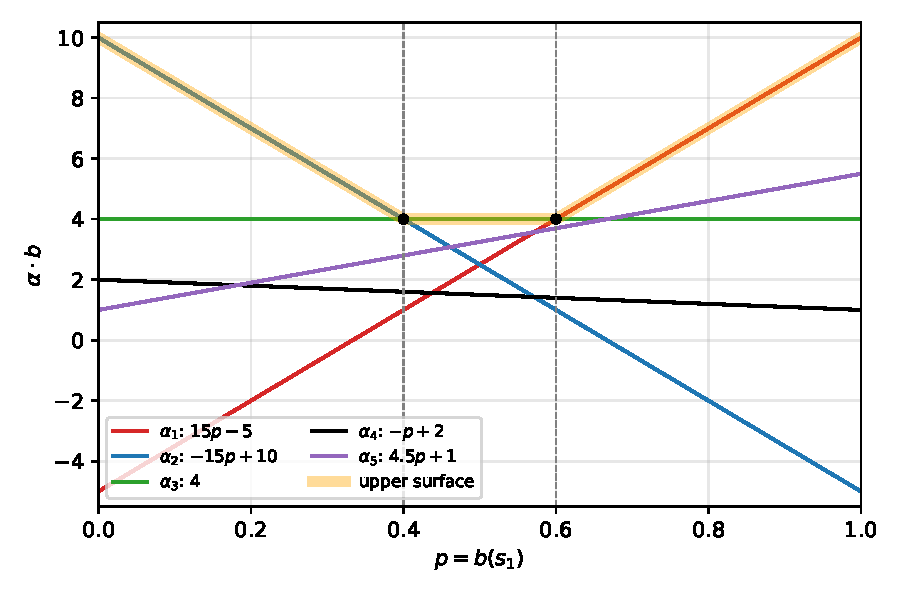
\includegraphics[width=0.7\linewidth]{figures/alpha_vectors.pdf}
  \caption{The five $\alpha$-vectors over $p\in[0,1]$ and the upper surface of $\Gamma$ (shaded), with breakpoints at $p=0.4$ and $p=0.6$.}
  \label{fig:alpha-vectors}
\end{figure}

\paragraph{(b) Pruning by pointwise dominance.}
From Figure~\ref{fig:alpha-vectors}, $\alpha_4$ and $\alpha_5$ lie strictly below the maximum for every belief $p\in[0,1]$, so both can be removed by pointwise dominance. The maximum is
\[
V_{\max}(p)=\begin{cases}
V_{\alpha_2}(p)=10-15p, & 0\le p\le 0.4,\\
V_{\alpha_3}(p)=4, & 0.4<p<0.6,\\
V_{\alpha_1}(p)=15p-5, & 0.6\le p\le 1.
\end{cases}
\]
For all $p\in[0,1]$, $V_{\alpha_4}(p)=2-p<V_{\max}(p)$ and $V_{\alpha_5}(p)=4.5p+1<V_{\max}(p)$. The dominating vector may differ with $p$. In contrast, $\alpha_1$, $\alpha_2$ and $\alpha_3$ each attain the maximum on an interval, so they cannot be removed.

% ---------------------------------------------------------------------
\subsection*{A3. Pedestrian avoidance: MDP vs POMDP}

\paragraph{Scenario where MDP is suitable.}
\begin{itemize}[nosep]
  \item S: [car\_position, pedestrian\_position]
  \item A: [Stay, Move]
\end{itemize}
Sensors accurately identify both positions. Assume movement is discrete and the next state depends only on the current positions and action. An MDP policy maps the observed state to the best action: if a pedestrian blocks the cell ahead, choose Stay; otherwise, choose Move when safe. Since the complete state is observed, a POMDP belief is unnecessary.

\paragraph{Scenario where POMDP is suitable.}
\todo{Describe the scenario, e.g.\ what part of the state the car cannot observe even with good sensors (pedestrian intention/destination?).}
\begin{itemize}[nosep]
  \item State (observed and hidden parts): \todo{}
  \item Observations: \todo{}
  \item Why reasoning over a belief changes the decision: \todo{}
\end{itemize}

% =====================================================================
\section*{Part B}
% =====================================================================

% ---------------------------------------------------------------------
\subsection*{B1. MDP framing of multi-drone navigation}

\begin{itemize}
  \item \textbf{State space} $S$: each state contains the positions of all $N$ drones, $s=(p_1,\dots,p_N)$, where $p_i=(x_i,y_i,z_i)$. 
  \item \textbf{Action space} $A$: A joint action $a=(a_1,\dots,a_N)$ specifies the simultaneous action of every drone. Thus, $A=A_1\times\dots\times A_N$ and $|A|=26^N$. For example, two drones have $26^2=676$ joint actions.
  \item \textbf{Transition function} $T(s,a,s') = T_{known}$
  \item \textbf{Reward function} for $N$ drones is the sum over all drones:
  \[
    R(s,a,s') = \sum_{i=1}^{N} R_i(s,a,s'),
  \]
  where
  \[
    R_i(s,a,s') = -1 + \begin{cases}
      -50, & \text{if drone $i$ collides},\\
      100, & \text{if drone $i$ reaches its goal}.
    \end{cases}
  \]
  \item \textbf{Discount factor} $\gamma$: \todo{e.g.\ 0.99}
\end{itemize}

% ---------------------------------------------------------------------
\subsection*{B2. Approximate on-line MDP solver}

\paragraph{Overview.} We use Monte Carlo Tree Search (MCTS) with UCT selection and a greedy rollout policy. At each decision step, the planner builds a search tree rooted at the current joint state within the available planning time (at most 10 seconds, without parallelisation). It estimates action values through sampled transitions and discounted returns, then executes a tried root action with the highest estimated value, breaking equal-value ties uniformly at random. Sampling avoids enumerating all possible successor states, although a large joint action space remains a limitation.

\subsubsection*{1. Selection}
At the current node, untried joint actions are sampled randomly and checked for valid intended moves. Once no eligible untried actions remain, select the tried eligible action with the highest Upper Confidence Bound (UCB):
\[
  a \leftarrow \arg\max_a\left[
    Q(\text{node},a)+\sqrt{\frac{2\ln N(\text{node})}{N(\text{node},a)}}
  \right].
\]
Here $Q(\text{node},a)$ is the estimated mean discounted return, $N(\text{node},a)$ is the number of times action $a$ has been tried at $\text{node}$, and $N(\text{node})=\sum_a N(\text{node},a)$. UCB balances actions with high estimated returns against actions that have been explored less often.

\paragraph{Validity checks and fallback.} \textsc{Safe}$(s,a)$ decodes the joint action and calculates each drone's intended target directly; a drone already at its goal keeps its current position. It returns true only if every target is inside the grid, outside obstacles and distinct from every other target. It does not call \texttt{env.simulate}, so stochastic outcomes can still collide. Invalid actions are cached at the node. Selection tests at most 64 randomly chosen untried candidates per call, then uses its cached greedy fallback if none passes or the deadline expires. The fallback is checked when first computed; if it is unsafe because no valid joint assignment exists, it is still returned. Tried actions considered by UCB have already passed the intended-target checks.

\subsubsection*{2. Expansion}
After selecting a joint action $a_i$ at $\text{node}$, call \texttt{env.simulate} to sample a successor joint state $s_j$, reward and terminal flag. Check whether the pair $(a_i,s_j)$ already exists among the children of $\text{node}$:
\begin{itemize}[leftmargin=*, itemsep=0.35em]
  \item \textbf{New pair:} Create a child node for $s_j$, initialise its action visit counts and values to zero, and store it under $(a_i,s_j)$.
  \item \textbf{Existing pair:} Reuse the stored child, move the search to that node and perform Selection again from there.
\end{itemize}
The parent is the node currently being visited; it is the root at the start of a search iteration. Because motion is stochastic, selecting the same action can produce different successor states, each stored as a separate outcome child. Tree descent continues through existing children until a new child is created, a terminal outcome is sampled, the depth limit \texttt{max\_num\_steps} is reached, or the planning deadline expires.

\subsubsection*{3. Rollout from a new node}
If the newly created child is nonterminal, start a rollout from its state using the greedy policy. Its simulated states are not added to the search tree. If the sampled outcome is terminal, skip the rollout. The total number of transitions in the tree and rollout is limited to $D=\texttt{max\_num\_steps}$: a child at depth $d$ has at most $D-d$ rollout steps remaining. The planning deadline also applies throughout.

\paragraph{Choosing a greedy action.} At each rollout step, process each drone that has not yet reached its goal:
\begin{enumerate}[leftmargin=*, itemsep=0.25em]
  \item For every available per-drone action vector $u$, calculate the intended candidate position $p_i+u$ directly. There are 26 vectors when altitude changes are enabled and 8 otherwise.
  \item Discard candidates outside the grid or inside an obstacle.
  \item Measure the Euclidean distance from each remaining candidate to that drone's goal $g_i$:
  \[
    \operatorname{distance}_i(u)=\lVert p_i+u-g_i\rVert_2.
  \]
  \item Order candidates from the shortest distance to the longest. Assign targets in drone order, trying the nearest candidate first. If a target is already assigned to another drone, try the next candidate; backtrack to an earlier drone's choice if necessary to obtain distinct targets for all drones.
\end{enumerate}
Drones that have reached their goals remain in place and occupy their goal cells. If no joint assignment with distinct, valid targets exists, the implementation uses its per-drone fallback choices, which are not guaranteed to avoid collision.

Candidate distances are calculated without calling \texttt{env.simulate} for every action. Only after choosing and encoding the joint action does the rollout call \texttt{env.simulate} once to sample the next state and reward. Because movement is stochastic, the sampled positions can differ from the intended candidates, so these checks cannot guarantee collision-free outcomes. Repeat greedy action selection from the sampled state until a terminal outcome, the remaining depth limit or the planning deadline is reached, accumulating discounted rewards.

\paragraph{Pseudocode so far.} Algorithm~\ref{alg:mcts-partial} shows one search iteration through the rollout call. Algorithm~\ref{alg:select} details \textsc{Select}, including validity checks, bounded sampling, fallback and UCB; Algorithm~\ref{alg:greedy-rollout} gives the rollout loop. \textsc{GreedyAction} follows the candidate-distance procedure above. Backpropagation is left for the next discussion.

\begin{algorithm}[H]
\small
\caption{One MCTS iteration: Selection, Expansion and rollout entry}
\label{alg:mcts-partial}
\KwIn{Root node, depth limit $D=\texttt{max\_num\_steps}$, planning deadline}
$\text{node} \leftarrow \text{root}$; $d \leftarrow 0$; $\text{path} \leftarrow [\,]$; $G \leftarrow 0$\;
\While{$d < D$ and time remains}{
  $a_i \leftarrow \textsc{Select}(\text{node},\text{deadline})$\;
  \If{deadline reached}{\textbf{break}\;}
  $(s_j,r,\text{done}) \leftarrow \texttt{env.simulate}(\text{node}.\text{state},a_i)$\;
  Append $(\text{node},a_i,r)$ to path; $d \leftarrow d+1$\;
  $k \leftarrow (a_i,s_j)$\;
  $\text{isNew} \leftarrow (k \notin \text{node}.\text{children})$\;
  \If{isNew}{
    $\text{child} \leftarrow \textsc{NewNode}(s_j)$ with all $N=0$, $Q=0$\;
    $\text{node}.\text{children}[k] \leftarrow \text{child}$\;
  }
  $\text{child} \leftarrow \text{node}.\text{children}[k]$\;
  \If{done}{\textbf{break} \tcp*{terminal outcome: no rollout}}
  \If{isNew}{
    $G \leftarrow \textsc{Rollout}(\text{child.state},D-d,\text{deadline})$\;
    \textbf{break}\;
  }
  $\text{node} \leftarrow \text{child}$ \tcp*{existing pair: repeat Selection here}
}
\end{algorithm}

\begin{algorithm}[H]
\small
\caption{\textsc{Select}$(\text{node},\text{deadline})$: choose a joint action}
\label{alg:select}
\KwIn{Node $\text{node}$ with state, visit counts $N$, values $Q$ and invalid-action flags}
\If{fallback has not been initialised at $\text{node}$}{
  $\text{node}.\text{fallback} \leftarrow \textsc{GreedyAction}(\text{node}.\text{state})$\;
  $\text{node}.\text{hasSafe} \leftarrow \textsc{Safe}(\text{node}.\text{state},\text{node}.\text{fallback})$\;
}
\If{not $\text{node}.\text{hasSafe}$}{\Return{$\text{node}.\text{fallback}$}\;}
$U \leftarrow \{a : N(\text{node},a)=0 \text{ and } a \text{ is not flagged invalid}\}$\;
\If{$U \neq \varnothing$}{
  $m \leftarrow \min(64,|U|)$\;
  \For{$j \leftarrow 1$ \KwTo $m$}{
    \If{deadline reached}{\Return{$\text{node}.\text{fallback}$}\;}
    Sample $a$ uniformly at random from $U$\;
    \If{\textnormal{\textsc{Safe}}$(\text{node}.\text{state},a)$}{\Return{$a$}\;}
    Flag $a$ invalid at $\text{node}$; remove $a$ from $U$\;
  }
  \Return{$\text{node}.\text{fallback}$}\;
}
$T \leftarrow \{a : N(\text{node},a)>0 \text{ and } a \text{ is not flagged invalid}\}$\;
\If{$T=\varnothing$}{\Return{$\text{node}.\text{fallback}$}\;}
$n \leftarrow \sum_{b\in T}N(\text{node},b)$\;
\Return{$\displaystyle\arg\max_{a\in T}\left[Q(\text{node},a)+\sqrt{\frac{2\ln n}{N(\text{node},a)}}\right]$}\;
\end{algorithm}

\begin{algorithm}[H]
\small
\caption{\textsc{Rollout}: discounted return using greedy actions}
\label{alg:greedy-rollout}
\KwIn{New child state $s$, remaining depth $L=D-d$, planning deadline}
$\hat{s} \leftarrow \text{copy}(s)$; $G \leftarrow 0$; $w \leftarrow 1$\;
\For{$t \leftarrow 1$ \KwTo $L$}{
  \If{deadline reached}{\textbf{break}\;}
  $a \leftarrow \textsc{GreedyAction}(\hat{s})$\;
  $(\hat{s},r,\text{done}) \leftarrow \texttt{env.simulate}(\hat{s},a)$\;
  $G \leftarrow G+w\,r$; $w \leftarrow \gamma w$\;
  \If{done}{\textbf{break}\;}
}
\Return{$G$}\;
\end{algorithm}

% ---------------------------------------------------------------------
\subsection*{B4. Empirical investigation of problem complexity}

\subsubsection*{Experimental setup}
\begin{itemize}[nosep]
  \item Hardware / Python version: \todo{}
  \item Planning time per step: \todo{}; max steps: \todo{}; $\alpha$: \todo{}; reward parameters: \todo{}
  \item Runs per scenario: \todo{$n$}; random seeds: \todo{}
  \item 95\% CI computed as $\bar{x} \pm t_{0.975,\,n-1}\, s/\sqrt{n}$ \todo{(or Wilson interval for success rate)}.
\end{itemize}

\paragraph{Performance metrics.}
\begin{itemize}[nosep]
  \item Success rate (all drones reach goal without collision)
  \item Total discounted reward
  \item Number of steps to completion (successful runs)
  \item Collision rate
  \item \todo{Tree statistics: simulations per step, average tree depth, etc.}
\end{itemize}

\paragraph{Complexity factors and how each is varied (one factor at a time).}
\begin{table}[H]
\centering
\begin{tabular}{p{2.8cm}p{5.2cm}p{6.6cm}}
\toprule
Set & Varied factor (others fixed) & What we expect to learn \\
\midrule
S: State space  & \todo{grid size, e.g.\ $5^3, 10^3, 15^3, 20^3$; drones fixed} & \todo{effect of longer horizons / sparser goal reward} \\
A: Action space & \todo{number of drones $N$ and/or altitude change (8 vs 26 per drone)} & \todo{effect of branching factor on search breadth} \\
C: Clutter      & \todo{number/density of obstacles, narrow passages} & \todo{effect on rollout quality and collision risk} \\
\bottomrule
\end{tabular}
\caption{Experiment design. \todo{Note that increasing $N$ also grows $|S|$; explain how the design separates the two factors.}}
\end{table}

\paragraph{Scenario list.}
\begin{table}[H]
\centering
\small
\begin{tabular}{llccccc}
\toprule
ID & Set & Grid & $N$ & Altitude change & \#Obstacles & $|A|$ \\
\midrule
S1 & S & \todo{} & \todo{} & \todo{} & \todo{} & \todo{} \\
S2 & S & \todo{} & \todo{} & \todo{} & \todo{} & \todo{} \\
S3 & S & \todo{} & \todo{} & \todo{} & \todo{} & \todo{} \\
A1 & A & \todo{} & \todo{} & \todo{} & \todo{} & \todo{} \\
A2 & A & \todo{} & \todo{} & \todo{} & \todo{} & \todo{} \\
A3 & A & \todo{} & \todo{} & \todo{} & \todo{} & \todo{} \\
C1 & C & \todo{} & \todo{} & \todo{} & \todo{} & \todo{} \\
C2 & C & \todo{} & \todo{} & \todo{} & \todo{} & \todo{} \\
C3 & C & \todo{} & \todo{} & \todo{} & \todo{} & \todo{} \\
\bottomrule
\end{tabular}
\caption{Testing scenarios. Config files in \texttt{\todo{experiments/configs/}}.}
\end{table}

\subsubsection*{Results}
\begin{table}[H]
\centering
\small
\begin{tabular}{lcccc}
\toprule
ID & Success rate (95\% CI) & Discounted reward (mean $\pm$ CI) & Steps (mean $\pm$ CI) & Sims/step (mean) \\
\midrule
S1 & \todo{} & \todo{} & \todo{} & \todo{} \\
S2 & \todo{} & \todo{} & \todo{} & \todo{} \\
S3 & \todo{} & \todo{} & \todo{} & \todo{} \\
\midrule
A1 & \todo{} & \todo{} & \todo{} & \todo{} \\
A2 & \todo{} & \todo{} & \todo{} & \todo{} \\
A3 & \todo{} & \todo{} & \todo{} & \todo{} \\
\midrule
C1 & \todo{} & \todo{} & \todo{} & \todo{} \\
C2 & \todo{} & \todo{} & \todo{} & \todo{} \\
C3 & \todo{} & \todo{} & \todo{} & \todo{} \\
\bottomrule
\end{tabular}
\caption{Summary statistics over $n=\todo{}$ runs per scenario.}
\end{table}

\begin{figure}[H]
\centering
\begin{subfigure}{0.32\linewidth}\centering
  \fbox{\parbox[c][3cm][c]{0.9\linewidth}{\centering\todo{plot}}}
  % \includegraphics[width=\linewidth]{figures/state_space.pdf}
  \caption{State space}
\end{subfigure}
\begin{subfigure}{0.32\linewidth}\centering
  \fbox{\parbox[c][3cm][c]{0.9\linewidth}{\centering\todo{plot}}}
  % \includegraphics[width=\linewidth]{figures/action_space.pdf}
  \caption{Action space}
\end{subfigure}
\begin{subfigure}{0.32\linewidth}\centering
  \fbox{\parbox[c][3cm][c]{0.9\linewidth}{\centering\todo{plot}}}
  % \includegraphics[width=\linewidth]{figures/clutter.pdf}
  \caption{Clutter}
\end{subfigure}
\caption{Mean discounted reward with 95\% CI error bars as each factor increases.}
\end{figure}

\subsubsection*{Discussion}
\paragraph{Effect of state-space size.} \todo{}
\paragraph{Effect of action-space size.} \todo{}
\paragraph{Effect of clutter.} \todo{}
\paragraph{Which factor degrades performance the most?} \todo{Answer, supported by the statistics (overlapping vs non-overlapping CIs, normalised degradation, etc.).}
\paragraph{Role of each solver component as complexity grows.}
\todo{Selection, expansion, rollout/heuristic, backpropagation, tree reuse: which helped or hurt, and why. Ablation results if run.}
\paragraph{Limitations and possible improvements.} \todo{}

% =====================================================================
\appendix
\section*{Appendix A: Generative AI disclosure}
% Required by the assignment: failure to disclose = cheating.
Tools used: \todo{tool names and versions, or ``None''}.

\noindent What they were used for: \todo{}

\noindent Full list of prompts:
\begin{enumerate}[label=\arabic*.]
  \item \todo{prompt 1 (verbatim)}
  \item \todo{prompt 2 (verbatim)}
\end{enumerate}

\section*{Appendix B: Additional results}
\todo{Optional: per-scenario raw tables, extra plots, ablations.}

% \section*{References}
% \begin{thebibliography}{9}
%   \bibitem{kocsis2006} L.~Kocsis and C.~Szepesv\'ari, ``Bandit based Monte-Carlo planning,'' ECML 2006.
% \end{thebibliography}

\end{document}
